\chapter{\label{chapter:stateofart}State-of-the-Art in Embedded Virtualization}

This section describes the current status of embedded virtualization. As shown in Chapter \ref{chapter:background}, hypervisors designed for general purpose virtualization cannot be directly adopted for ES. However, this chapter starts by showing well-known hypervisors widely used for cloud computing. They present larger footprints and overheads than hypervisors that are specially designed for embedded systems. Several authors have dedicated their work to adapting them for ES. The chapter is divided into the following sections:  Subsection \ref{section:xen} presents the architecture and proposals based on the Xen hypervisor. Xen was designed for enterprise appliances. Therefore, there are ports for embedded devices and special support for real-time. Subsection \ref{subsection:kvmproposals} presents proposals based on KVM (Kernel-Based Virtual Machine), a type 2 hypervisor, which was ported for the ARM architecture. The remaining hypervisors that will be presented were developed for  ES. Section \ref{section:spumone} describes the SPUMONE hypervisor. Section \ref{section:XtratuM} presents XtratuM, a hypervisor for safety critical systems. Section \ref{section:l4} presents three different embedded hypervisors based on the L4 microkernel family: OKL4, L4/Fiasco, PikeOS and Mini-Nova. Section \ref{section:mhyper} presents the M-Hypevisor. Section \ref{section:xvisor} shows the XVisor embedded hypervisor. A comparative study between the hypervisors is presented in Section \ref{section:comparative}. Section \ref{section:rtlinux} explains how the RT-Linux patch modifies the Linux kernel and how it is similar to virtualization. Finally, Section \ref{section3:considerations} concludes this chapter. 


\section{The Xen Hypervisor}
\label{section:xen}

Xen is an open-source type 1 hypervisor that has been developed over the last 13 years \cite{xen2003}. Today, Xen is used for different commercial and open-source projects, such as: server virtualization, desktop virtualization, security and embedded applications. Additionally, Xen supports the largest clouds in production today\footnote{http://www.xenproject.org/}. Initially developed for desktop or server application, it was modified to be embedded, especially for ARM processors.

\subsection{Xen's Architecture}
\label{subsubsection:xenarch}

Figure \ref{fig:xenarch} depicts Xen's architecture. Xen is responsible for handling CPU, memory, interrupts and scheduling the VMs. Xen is a type 1 hypervisor, thus, it interacts directly with the hardware and the VMs executes over it. A running instance on a VM in Xen is called domain or guest. There is a special domain, called \emph{Domain 0} (Dom0), that is responsible for I/O and also contains a stack to manage the VM’s creation, destruction and configuration, called \emph{Toolstack}. 


\begin{figure}[!hbtp]
\centering
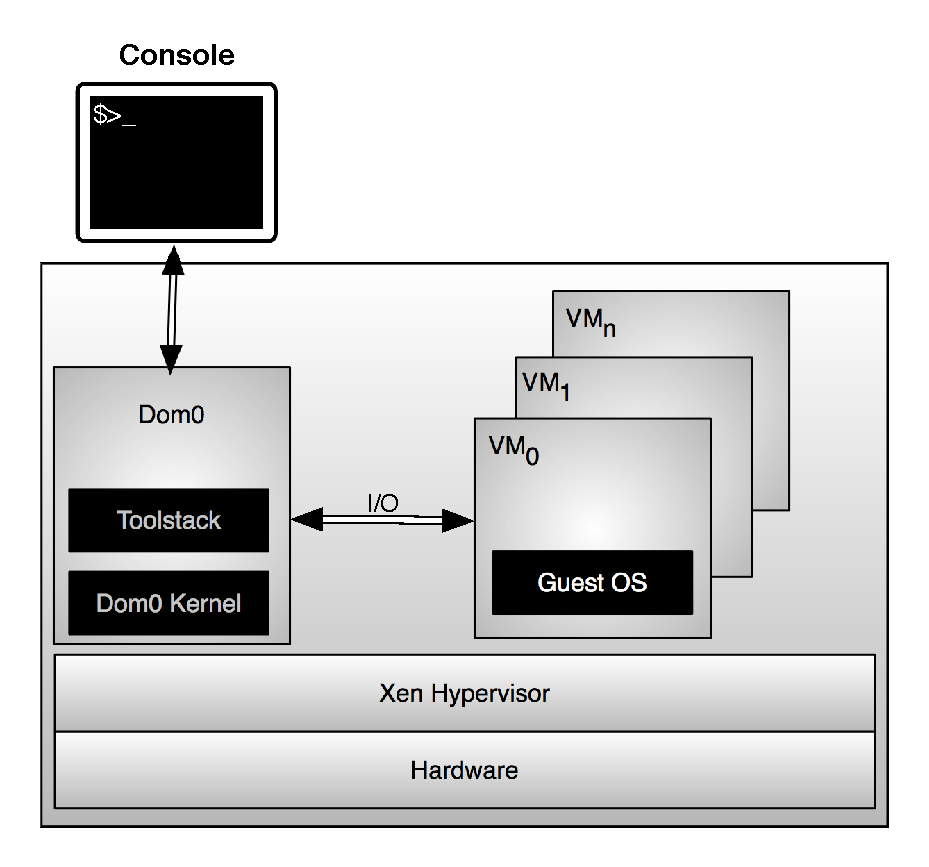
\includegraphics[width=.45\textwidth]{./chapter3/figures/xenarch}
\caption{Xen's Architecture. Adapted from \cite{xen2003}.}
\label{fig:xenarch}
\end{figure}

The Xen hypervisor has less than 150,000 lines of code and a footprint around 600KB. However, the footprint can variate with different compilers and compilation flags. Xen does not implement I/O functions such as networking or storage itself. Instead, I/O functionality is accomplished by the Dom0. Dom0 has special privileges to access the hardware directly and it is responsible for handling the I/O for all VMs. Thus, if a VM needs an I/O function it must interact with Dom0, which will execute the transaction with the hardware. Additionally, the Dom0 implements the Toolstack, which exposes an interface composed of the command line and graphical interface, as well as interacts with cloud APIs like OpenStack \cite{openstack} for configuration purposes.

The Xen architecture requires that the guests are modified (patched), since all I/O are redirected to Dom0. Essentially, Xen was designed to be a para-virtualized hypervisor. Therefore, this approach prevents  unmodified guest OSs be virtualized on top of Xen. Thus, proprietary OSs like Microsoft Windows can not be virtualized. Aiming to overcome this limitation, Xen implements the hardware-assisted virtualization (HVM) that uses virtualization extensions from the CPU, like Intel VT or AMD-V. Xen does not deal with I/O directly, thus, it needs to use the Qemu \cite{qemu} to emulate BIOS, IDE disk controller, VGA graphics adapter among others devices. This allows for Xen to perform full-virtualization. However, the device emulation causes a performance issue and fully-virtualized guests over Xen are usually slower than the para-virtualized ones. Nonetheless, Xen provides a technique to avoid the performance issue when using HVM, called PV on HVM. This technique consists in to combine para-virtualization and full-virtualization. Thus, para-virtual device drivers are installed in the guest OS to bypass the emulation for storage and network I/O. CPU and memory virtualization continues to be performed by hardware support. This allows for performance improvement for guest proprietary or even open source OSs. However, it requires the implementation of para-virtual device drivers to the guest OSs. Both PV and HVM guests can coexist on a single Xen system.

\subsection{The Xen Scheduling Algorithm}
\label{subsubsection:xensch}

An important component of a hypervisor is the scheduler. The default Xen's scheduler is called Credit Scheduler \cite{Ding2014}. Xen implements two other scheduling algorithms: the Simple Earliest Deadline First (SEDF) \cite{sedf} and the Borrowed Virtual Time (BVT) \cite{Duda:1999}. Although at the present time both algorithms are available, they are marked as deprecated and probably they will be removed from the Xen's source code. Nevertheless, several works still rely on SEDF to improve real-time on XEN. Thus, just the Credit Scheduler and the SEDF will be discussed. 

In the Credit Scheduler, each domain has two special attributes: weight and cap. The weight determines the proportional fair share of CPU resource. For example, a domain with weight of 1024 will get the CPU two times more than a domain with weight of 512. The weight values range from 1 to 65535 and the default is 256. The cap is an optional parameter used to determine the amount of CPU that a domain will be able to consume, even if the host system has idle CPU cycles. The cap is expressed as a percentage of one physical CPU. For example, a cap of 0.5 means that the domain can take up to 50\% of CPU time, 1 means the domain can take upto 100\% of the CPU time and 2 means the domain can take upto 100\% of two CPUs' time. When cap is 0 means there is no limit for CPU usage.  Credit scheduler keeps a local queue of runnable VCPUs by physical CPU ordered by priority. When a VCPU is scheduled, the algorithm computes how much time (credits) was consumed and subtracts from the total time reserved for it. If the VPCU exceeds its available credits it is in "over" status, otherwise, it is in "under" status. Once in over status, the VCPU needs to wait for the next period to execute again. By default, the scheduler quantum is 10ms and the VCPU credits are recomputed each 30ms. In a SMP platform, when a CPU does not find a VCPU in under status in its local queue, it looks on other CPU queues for one. This is called SMP load balancing and it guarantees that there is not an idle CPU when there are runnable VPCUs in the system.

The SEDF scheduler allows to allocate processing resources for each domain according to period, deadline (the time when the period ends) and capacity (the amount of processing time reserved to the domain in a period). In fact, the algorithm guarantees that a domain will be executed for the amount of time given by its capacity on each time interval given by its period \cite{Ongaro2008}. The algorithm keeps the deadline for each domain and the amount of processing remaining to be done before the deadline. The domains are sorted in the execution queue according to their deadlines. An interesting effect of this algorithm is that when a domain consumes processing time, its deadline will be moved forward. Thus, I/O-intensive domains that consume little processing time will typically have earlier deadlines, which means higher priority over CPU-intensive domains. This is advantageous to environments that combine CPU and I/O intensive domains. The main disadvantage of the SEDF algorithm is to keep local queues organized by CPU on multicore processors preventing VCPU migration across multiple cores and avoiding dynamic workload balance. Nevertheless, it was made obsolete because with Credit scheduler is possible to improve scheduling performance on multiprocessors.


\subsection{Xen-Based Proposals}
\label{subsubsection:xenproposals}

The proposals to improve real-time responsiveness on Xen hypervisor are typically based on two different approaches: a) improving the Xen's scheduler real-time responsiveness, or; b) dealing with the hierarchical scheduling problem. The first approach typically tries to improve the real-time scheduler responsiveness by applying different scheduling algorithms or non-intrusive techniques to monitor the guest’s behavior. Nevertheless, such approaches generally do not consider the hierarchical scheduling problem. The second approach uses theoretical research on hierarchical real-time scheduling or intrusive techniques that require modifications inside of  the guest OSs.

\subsubsection{Improving The Scheduler's Real-time Responsiveness}

Ongaro et al. \cite{Ongaro2008} studied the performance impact on the Xen hypervisor when multiple guests with different workloads (CPU-intensive, I/O-intensive and latency-sensitive) run concurrently. The results led to some optimization proposals, including disabling preemption for Dom0 and sorting the scheduler run queue based on the remaining credits  to give priority to I/O-intensive domains. These optimizations were focused on improving the I/O performance, nevertheless, the authors claim that it impacts latency positively. Finally, their study showed that latency-sensitive applications will perform better when not combined in the same domain with CPU-intensive applications. Instead, latency-sensitive applications should be placed within their own domain. 

Lee et al. \cite{Lee2010} introduced the laxity concept enhancing the soft real-time performance of the Xen Credit scheduler. Each domain has an attribute named laxity used to define the position where its VCPUs will be inserted in the scheduler's run queue. In other words, it is possible to use laxity to determine the maximum desired latency for a real-time domain, because when a VCPU is inserted into the run queue, it is inserted where its deadline is expected to be met. 

Masrur et al. \cite{Masrur2010} implemented a new scheduler for Xen based on the SEDF scheduler aiming to improve its worst-case response time, named  \emph{Priority-based scheduling plus SEDF} (PSEDF). The major difference is that PSEDF implements the concept of real-time domains (domRT), where, a domRT has scheduling priority over non real-time ones (domU). When several domRTs coexist at the same Xen instance, priorities must be defined between them. The domUs continue to be scheduled with the default SEDF. The resulting scheduler allows safety-critical applications (e.g. airbag control and brake system) to be run on the same hardware with general-purpose applications (e.g. navigation and multimedia). The main drawback of the authors’ technique is that a domRT can just contain a single real-time application to avoid the hierarchical scheduling problem.

Hu et al. \cite{Hu2010} proposed a technique to improve the I/O performance of Xen on multicore processors. Their technique take advantage of the fact that traditional hypervisor schedulers, including Xen, focus on sharing the processor's resources fairly among domains, while, the scheduling of I/O resources is treated as a secondary problem. This seriously impacts on the performance of applications that execute I/O-intensive tasks, like network or storage. The authors’ technique consists of implementing  a scheduler for multicore dynamic partitioning, where, the processor cores are divided into three specialized subsets with different scheduling strategies. The subset called driver core host only the dom0, i.e, the dom0 is bounded to a physical core and never is scheduled. The fast-tick cores subset handles I/O events and its scheduler employs small time slices to ensure fast response to I/O events. Finally, the general cores subset is used for computation-intensive workloads. Their approach increases I/O performance, although, it degrades the performance for CPU-intensive applications.

Huacai et al. \cite{huacai2010} proposed improvements to Xen's Credit scheduler from the real-time perspective to guarantee audio performance (avoiding human-sensible glitches) in virtualized environments. Their strategy consist of three approaches: flexible time slices, real-time priority adjustment and adaptive audio-aware. The Credit scheduler was modified to allow flexible time slices, i.e, the scheduler restriction of fixed time slices or quantum of 10ms (see Subsection \ref{subsubsection:xensch}) was removed allowing different time slice lengths. For example, a real-time domain may receive 1ms time slice and a non real-time may receive the default time slice (10ms).  The real-time priority adjustment promotes a domain from non real-time to real-time when the user plays audio. The adaptive audio-aware algorithm is used to detect when the user starts/stops the audio player given to it a higher priority. 

Credit scheduler was designed to be efficient with computation intensive workloads. However, I/O-intensive tasks suffer from latency issues. To minimize this problem, Zeng et al. \cite{zeng2013} enhanced performance to the I/O latency-sensitive applications minimizing the system response time by balancing the VCPUs with BOOST priority in multi-core systems. BOOST is an additional priority level of the Credit scheduler, which allows a VCPU to preempt a running VCPU in under state. The results showed that their proposal can improve the response time for latency-sensitive applications without having adverse impact on compute-intensive applications. 
 
Cheng et al. \cite{cheng2015} optimized the Xen's scheduler for soft real-time applications. They introduced a new priority level marking high priority VMs as real-time domains. Additionally, their strategy includes management of the physical CPU's queue, limiting the number of real-time domains to guarantee to meet the scheduling requirements, and pinning VCPUs to physical CPUs to reduce the performance impact caused by VCPU migration. The authors evaluated their solution using IP telephony workloads for soft real-time applications. The results compared to Credit scheduler and RT-Xen showed that their purpose achieves best performance and maintains a fairer scheduling in the meantime.

\subsubsection{Dealing With The Hierarchical Scheduling Problem}

Masrur et al. \cite{Masrur2011} proposed the design of a scheduler to deal with the hierarchical scheduling problem targeting automotive applications. The authors consider that all domains schedule their applications using the deadline-monotonic scheduler algorithm. On the other hand, the hypervisor utilizes the rate-monotonic scheduler algorithm \cite{Buttazzo2005} \cite{brun2015} for VCPU scheduling. Thus, they proposed a method to determine optimum time slices and periods for each VM in order to maintain their time constraints. The proposed scheme was validated using the Xen hypervisor. Their solution solves the hierarchical scheduling problem without hypercalls between the VM and hypervisor, although the Xen's default scheduler algorithm must be modified to accommodate the rate-monotonic algorithm. 

The RT-Xen project \cite{sisu2011} implements a hierarchical scheduling architecture based on fixed-priority scheduling focused on soft real-time applications for single-core processors. It considered four fixed-priority scheduling policies for the RT-Xen scheduler: Deferrable Server \cite{strosnider1995}, Sporadic Server \cite{sprunt1989}, Periodic Server and Polling Server \cite{sha:1986}. The four scheduling policies were implemented and compared to Xen's Credit Scheduler and SEDF schedulers. The experiments was conducted using a modified kernel Linux implementing the rate-monotonic scheduling algorithm. The results show that RT-Xen presents an acceptable soft real-time performance. The Deferrable Server presented the best results, while the Periodic Server suffered from a high number of missed deadlines in overloaded situations. Recently, it was released the RT-Xen 2.0 \cite{sisu2014} supporting multi-core processors and up to eight combinations of real-time VM scheduling policies. Moreover, it supports a range of interfaces for compositional scheduling, which enables designers to calculate and specify the resource demands of VMs to the underlying RT-Xen 2.0 scheduler. 

Lee et al. \cite{Lee2012} proposed a Compositional Scheduling Architecture (CSA) that enables timing isolation among VMs and supports timing guarantees for real-time tasks running on each VM. The CSA supports a broad range of real-time scheduling algorithm at the hypervisor level, and it was implemented extending the original RT-Xen interfaces. The authors presented an extensive evaluation to demonstrate the utility and effectiveness of CSA in optimizing real-time performance. The results using both synthetic and avionics workloads showed significant improvements regarding response time.

Yoo et al. \cite{seehwan2014} studied the schedulability in VMs considering the quantization overhead caused by the Xen's scheduler. Quantization overhead comes from tick-based scheduling of Xen-ARM, which requires integer presentation of scheduling period and execution slice. To minimize the quantization overhead they proposed a new algorithm to provide accurate and efficient parametrization of real-time VMs. Next, they presented an inter-VM schedulability test to the real-time VMs. Their proposal was evaluated on an ARM platform using a RTOS. Their experiments showed that is possible to guarantee the deadline for real-time tasks scheduled in a hierarchical fashion. However, the SEDF scheduler must be used as Xen's scheduler. Moreover, their work does not cover the I/O, since it is complex in Xen and requires a separate investigation. 

\subsubsection{Other Proposals}

Avanzini et al. \cite{avanzini2015} proposed the integration of the ERIKA OS\footnote{http://erika.tuxfamily.org/drupal/} and the Linux on a dual-core processor through Xen. ERIKA OS is an open-source, low-footprint and real-time operating system certificated for automotive applications. Their system configuration consisted in the Linux as dom0 and ERIKA OS as domU. The system was prototyped on a cubieboard2\footnote{http://cubieboard.org/}, an ARMv7 with virtualization extensions. In their proposed setup, each of the domains runs on a dedicated core, assigned statically by the hypervisor. Linux is the control domain, thus performing the Xen toolstack. Moreover, it must grant to ERIKA access to any I/O-memory range needed. Their approach provides an improved temporal isolation of concurrent operating systems. The main drawback is to keep the guests on dedicated cores not allowing load-balancing. 

\section{KVM Hypervisor}
\label{section:kvm}

The Kernel-based Virtual Machine (KVM) is a type 2 hypervisor designed to be a kernel-resident virtualization infrastructure, meaning it is totally integrated with the Linux Kernel since the 2.6.20 release. KVM is implemented as a Linux kernel module providing full-virtualization when hardware-assisted virtualization is supported, otherwise it provides para-virtualization. It supports SMP hosts and guests and enterprise level features like live migration\footnote{http://www.ibm.com/developerworks/library/l-hypervisor/}, which is the ability to move guest OSs between physical servers.

\subsection{KVM's Architecture}
\label{subsection:kvmarch}

KVM's architecture is shown in Figure \ref{fig:kvmarch}. It is composed of two main components: the KVM-loadable module that manages the virtualization hardware and exposes a configuration interface through the /dev file system; and a modified version of Qemu, called qemu-kvm, used to provide platform peripheral emulation. 

\begin{figure}[hbtp]
\centering
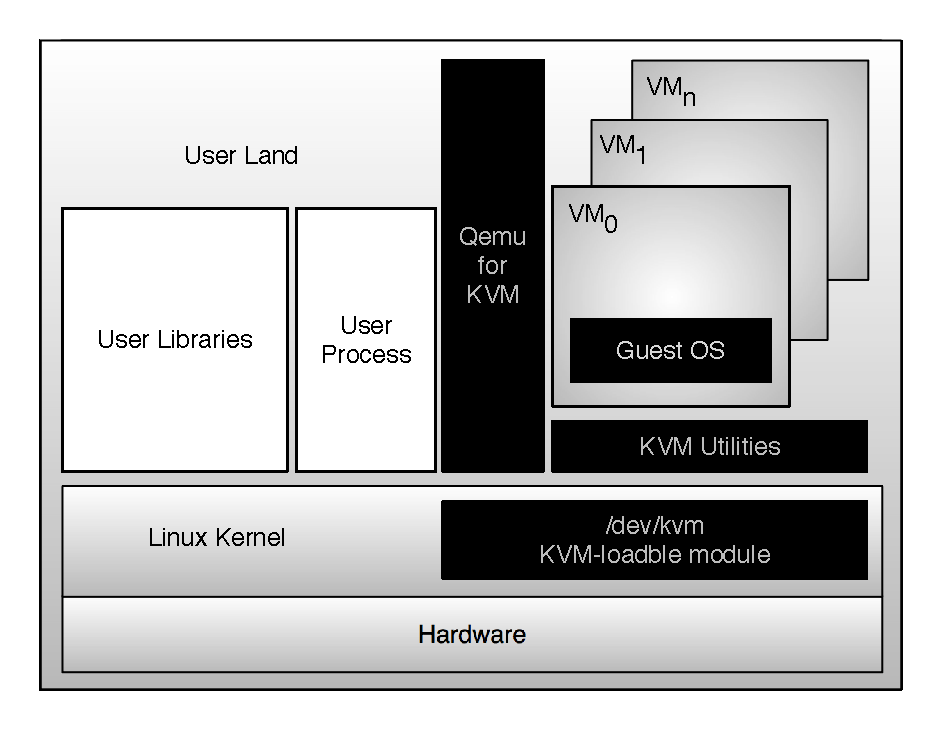
\includegraphics[width=.45\textwidth]{./chapter3/figures/kvmarch}
\caption{KVM's Architecture.}
\label{fig:kvmarch}
\end{figure}

A utility called kvm is used in user land to boot a guest OS in KVM. Once booted, the guest becomes a process of the host OS being scheduled like any other process by the Linux scheduler. Each VM has its own virtual memory space mapped to the host's physical address. Nevertheless, I/O requests are mapped through the host kernel to the Qemu for emulation purposes. Although KVM is strongly dependent of the Linux OS, it supports a rich list of guest OSs which includes Linux distributions, Microsoft Windows, QNX, Solaris x86, FreeBSD among others. 

KVM is mature enough to support advanced enterprise features such as enhanced security and live migration. Security in Linux is based on the Security-Enhanced Linux (SELinux) \cite{redhat}, which is  a project developed by the NSA to add access control, multi-level and multi-category to the kernel.   From the Linux kernel point-of-view, a guest OS is like any other process, it is possible to apply the standard Linux security model over it. Thus, SELinux can be used by the administrator to define permissions assuring that a VM resource can not be accessed by any other process or VM.  Nonetheless, with live migration, a VM can be moved between physical servers transparently to the end user. 

Similar to Xen (see Subsection \ref{subsubsection:xenarch}), KVM implements a mix of para-virtualization and full-virtualization in order to speed up I/O operations. Para-virtualized device drivers are installed in the guest OS in order to avoid the necessity of Qemu emulation for certain devices, specially networking and block devices. Nevertheless, KVM implements a standard called VirtIO (developed by IBM and Red Hat in conjunction) \cite{Russell2008}, which is an independent interface for building device drivers to offer better interoperability between hypervisors. When a hypervisor uses a proprietary interface for para-virtualized device drivers the guest is not portable between different hypervisors. VirtIO improves the portability of guests between hypervisors. 

\subsection{The Linux Scheduling Algorithm}
\label{subsubsection:linuxsch}

KVM does not have its own scheduler, instead, it takes advantage of the Linux scheduler. Therefore, a minimal background in Linux scheduling is necessary  to understand how real-time is addressed by KVM. The Linux OS is a general purpose OS. Thus, the scheduling algorithm has a set of requirements with conflicting objectives: good throughput for background jobs, avoidance of starvation, dealing with high and low priority processes, among others. The Linux scheduler implements a set of rules, called scheduling policy, that determine how a process will be scheduled. In order to apply a scheduling policy onto a process the scheduler needs to classify the process according three different process classes:

\begin{itemize}
\item \emph{Interactive}: Processes that interact constantly with the user. These processes spend a lot of time waiting for user inputs. Once, the input is received, it must return a quickly response or the user will consider the system unresponsive.
\item \emph{Batch}: Processes running in the background and that do not need user interaction. 
\item \emph{Real-time}: Processes with very strict scheduling requirements. 
\end{itemize}

Linux 2.6 and higher implement a sophisticated heuristic algorithm based on the past behavior of the processes to classify they as interactive or batch. The scheduler gives priority to interactive processes over batch ones \cite{bovet}, which results in a better response time even when the system is running under a heavy load. Real-time processes need special attention and there is a set of kernel features that improves the real-time responsiveness. In fact, improvements in the KVM real-time response implies on improvements in the Linux real-time response. 

Conventional processes (non real-time) have an attribute value called static priority which determines the time quantum of the process following the Equation \ref{eq:quantum}. The legal range for static priority is from 100 (highest priority) to 139 (lowest priority). As a consequence of Equation \ref{eq:quantum}, higher priority processes get longer slices of CPU time.


\begin{equation}
\label{eq:quantum}
quantum = \left\{\begin{matrix}
(\text{140 - static priority)} \times \text{20} & \text{if static priority} < \text{120}) \\
(\text{140 - static priority)} \times \text{5} & \text{if static priority}  \geq \text{120})
\end{matrix}\right.
\end{equation}

In addition, a conventional process also has a dynamic priority which is the number actually used by the scheduler to choose the next process to run. The dynamic priority is determined by the Equation \ref{eq:dyn}. 

\begin{equation}
\label{eq:dyn}
\text{dynamic priority = max (100, min(static priority - bonus + 5, 139))}
\end{equation}

The bonus variable is determined by the process'  average sleep time, that is, the average time (in nanoseconds) spent by the process while sleeping. The average sleep time is not allowed to be greater than 1 second. Each interval of 100 milliseconds represents a bonus value. For example, an average sleep time between 0 and 99 milliseconds results in a bonus equal to 0, intervals between 100 and 199 result in a bonus of 1. The greatest bonus value is 10. Nonetheless, the average sleep time is used by the scheduler to determine if a process is considered interactive or batch. If a process satisfies Equation \ref{eq:int}, it is considered interactive.

\begin{equation}
\label{eq:int}
\text{dynamic priority} \leq  \text{3} \times \text{static priority} / \text{4} + \text{28}
\end{equation}

A real-time process has an attribute called real-time priority with a legal range from 1 (highest priority) to 99 (lowest priority). Their main difference from conventional processes is that a real-time process inhibits the execution of every lower-priority process while it remains runnable \cite{bovet}. Nevertheless, if several real-time process with the same priority are ready to run at same time, the scheduler will choose the process that occurs first in the runnable queue. Hence, there is no time reservation and no guarantee that a process will be scheduled at a certain time. The user must explicitly set the process to the real-time state using the system calls sched\_setparam() and sched\_setscheduler().


\subsection{KVM-based proposals}
\label{subsection:kvmproposals}

As previously explained, a VM in KVM is treated as a Linux process, hence, any real-time improvement to the Linux host scheduler will translate in real-time improvement to the VM. Yet, other approaches are possible such as adding hypercalls to allow a guest OS to dynamically boost the priority of its VCPUs or implement a hierarchical scheduling algorithm scheme in both the host and guest OSs. 

Kiszka \cite{kiszka2009} analyzed the KVM real-time responsiveness in two situations: 

\begin{itemize}
\item  Qemu/KVM running onto a Linux kernel with CONFIG\_PREEMPT, which is  a compilation flag that allows the Linux kernel to be preemptive resulting in better responsiveness;
\item  The same configuration plus the PREEMPT-RT kernel patch. PREEMPT-RT is a kernel patch that improves the Linux kernel real-time responsiveness.
\end{itemize}
Based on the results, the authors proposed real-time improvements to KVM given higher priority to the qemu-kvm thread and to the desired VCPUs at the expense of giving lower priorities to other Linux processes. Additionally, a para-virtualized scheduling approach was implemented consisting of two hypercalls: set scheduling parameters (used to change a VCPU priority) and, interrupt done (used to indicate that its interrupt handling is done and no reschedule is required). These hypercalls allow the guest to adjust its priorities according to  the task currently running.  Nevertheless, this implies that KVM cannot be executed as a strict full-virtualization system. The results showed that when using PREEMPT-RT kernel patch, the guest can achieve better determinism and sub-millisecond scheduling latencies. Yet,, the hypercall scheme introduced up to 25\% higher average latencies.The authors claim that this impact could be reduced by optimizing their approach. 


Cucinotta et al. \cite{cucinotta2009} proposed the use of mechanisms designed according to the theory of hierarchical scheduling on real-time systems aiming to enhance predictability of the temporal behavior of VMs. They offered two different approaches: fixed priority (FP) inter-VM scheduling and reservation-based inter-VM scheduling. The first approach considers that the hierarchy is FP/FP, i.e, fixed-priority scheduling in both the hypervisor and guest OS scheduler.  In the second approach, they implemented a variant of the Constant Bandwidth Server (CBS) scheduler algorithm \cite{abeni1998}. Introduced by \cite{Palopoli2009}, this variant consists of a modification to ensure hard time reservation behavior at the hypervisor level and keeping the fixed-priority scheduling in the guest OS. The authors used KVM to validate their approach without considering the influence of the virtualized I/O. The results show that the hierarchical real-time scheduling theory may be effectively applied to virtualized systems. In \cite{cucinotta2011}, Cucinotta et al. addressed the problem of providing network response guarantees to VMs on multicore hosts. Their proposal is focused in single-core VMs scheduled according to a partitioned EDF policy, meaning that each VM is pinned to a certain CPU. The EDF scheduler algorithm provides  time isolation between VMs resulting in a significant delay time when asynchronous events occur, e.g., when a network packet is received and the VM is in the non-responsive time frame. In order to avoid delays imposed by the EDF scheduler and improve the responsiveness for network traffic, the authors modified the original EDF algorithm adding spare time to the VMs. The spare time is used by a VM when it exhausted its time budget, thus, the VM is allowed to execute for a short time being able to receive and eventually respond to network traffic. The results show a significant response time increase for network traffic. 

Zuo et al. \cite{zuo2010} studied the behavior of a virtualized RTOS running on KVM. A way to minimize the average latency on the RTOS is to increase its priority over the other Linux processes. This approach affects negatively the whole CPU throughput. However, the authors claim that usually the execution of RT tasks is short or periodic, thus, the RTOS do not always need to have higher priority. Based on this affirmation, hypercalls are introduced allowing the guest to inform its priority to the host. Thus, if a guest is going to enter a time-critical execution, it informs the host about the desired scheduling policy and priority. When no more time-critical execution necessary, the guest informs to the host to lower its priority. 

RESCH (Real-time Scheduler) framework \cite{kato2010} is a loadable kernel module (RESCH core) and a user library (RESCH library) that allows for the  implementation of new scheduling algorithms within Linux without modifying the kernel. Asberg et al. \cite{asberg2011} implemented a hierarchical scheduler using RESCH and applied it to both host and Linux guest. As result, it is possible to have a two layer scheduler approach that does not require kernel modifications. Instead, only RESCH kernel and libraries must be installed on both the host and guest. The advantage of this approach is that it is not restricted to KVM, i.e, it can be applied at any other virtualization layer, like VirtualBox \footnote{https://www.virtualbox.org/}. The authors claim that their approach can improve performance of multimedia intensive applications, because the CPU availability for video and audio can be better controlled. 

Yunfang et al. \cite{Yunfang2013} proposes the KVM-Loongson, a virtualization solution for MIPS based on KVM to the Loongson-3A \cite{loogson3a} processor. This processor do not implement the recently released MIPS virtualization extensions. Nonetheless, MIPS without the VZ module does not allow full-virtualization because it cannot support complete virtualization of kernel virtual address space. A possible solution targeting full-virtualization is to modify the processor core as presented at \cite{VHH_MIPS4Kc}. However, the authors modified the KVM (primarily designed for full-virtualization) to support para-virtualization. The authors performed an intensive study to determine all Linux kernel privileged instructions that could be substituted by hypercalls. As a result, they showed that about 98.6\% of the privileged instructions can be substituted. Still, their memory virtualization overhead is about 4\% on average. The main disadvantage of their technique is the effort to para-virtualize the Linux kernel and the impossibility to support proprietary software. 

Dall and Nieh \cite{Dall2014} proposed a KVM port to the ARM architecture with virtualization extensions, called KVM/ARM. This architecture takes the advantage of the wide Linux hardware support to the ARM family to simplify the hypervisor development and maintenance. It became the standard ARM hypervisor for Linux platforms. Experimental results showed an average of 10\% overhead when compared to native execution and significantly lower overhead when compared to KVM x86 virtualization. KVM was designed for general-purpose computing. Therefore, it does not comply with ES constraints like small footprint and real-time. For example, KVM/ARM requires a native Linux as host increasing the minimal system memory footprint. Additionally, KVM/ARM relies on the Linux OS scheduler which means it is difficult to improve the real-time responsiveness on virtualized OSes. 

Zhang et al. \cite{Dan2015} used the KVM/ARM to explore virtualization with a promising kind of main memory: non-volatile random access memory (NVRAM). This technology has attractive features, such as high density and low standby power. However, it has a long write latency that slow down the performance of write-intensive applications. Thus, time-critical tasks may result in unacceptable performance. The authors focused on improving the embedded virtualization with NVRAM/DRAM hybrid main memory. They proposed the NV-CFS, an optimized scheduling method that includes two main elements: a task allocator and a VM scheduler. The task allocator place write-intensive tasks in DRAM and read-intensive tasks in the NVRAM. The VM scheduler improves the system performance by giving a higher priority to foreground VMs. Thus, focusing on the user experience. Their approach can improve the performance by at least 30\% when compared to the same system without NVRAM. In addition, they claim a reduction on task deadline misses ratio compared to the original scheduling algorithm. 


\section{SPUMONE}
\label{section:spumone}

Kanda et al. \cite{spumone2008} proposed a lightweight virtualization layer for embedded systems called SPUMONE (acronym for Software Processing Unit, Multiplexing ONE into two). SPUMONE builds a hybrid operating system environment composed by a RTOS running in parallel with a GPOS, i.e., multiplexing the CPU between the OSs. SPUMONE's architecture is shown in Figure \ref{fig:espumone}. It was designed to address three main goals:

\begin{itemize}
\item minimal code modification on the guest OS, since it uses the para-virtualization technique;  
\item the hypervisor should be as light as possible; 
\item reboot the guest OSs independently from each other. 
\end{itemize}

SPUMONE supports just the SH-4A \cite{sh4a} architecture and virtualizes only the CPU, i.e., it does not implement peripheral virtualization (a peripheral must be mapped directly to a guest OS). In order to minimize the engineering cost of modifying the guest OS and improve performance, both the hypervisor and guest OSs run in privileged mode. Thus, most of the privileged instructions are executed directly and just minor instructions are replaced by hypercalls. The GPOS can provide isolation between user applications, since they run in the unprivileged mode. Nevertheless, the hypervisor, RTOS and GPOS run in the privileged mode without memory isolation. A fault in one of these three software components may compromise the entire system. 

\begin{figure}[!hbtp]
\centering
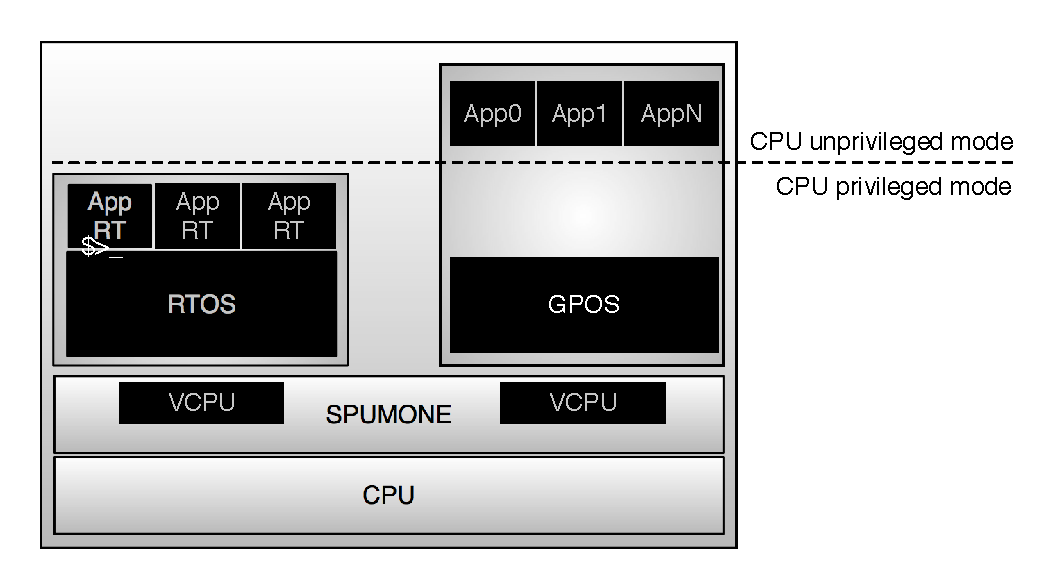
\includegraphics[width=.55\textwidth]{./chapter3/figures/spumone}
\caption{SPUMONE's single-core Architecture. Adapted from  \cite{spumone2008}.}
\label{fig:espumone}
\end{figure}

Mitake et al. \cite{hitoshi2011} proposed a distributed multicore architecture for SPUMONE as depicted in the Figure \ref{fig:espumone_multi}. Each CPU runs a SPUMONE instance and all guest kernels run at the privileged level. Each instance keeps a local memory area for data accessible only from local CPU. The authors claim that this design can reduce the intrusion risks at the virtualization layer, because a hypervisor instance is limited to one CPU. Additionally, this reduces the need of shared structures and synchronization among instances  increasing the scalability of the system. 

\begin{figure}[!hbtp]
\centering
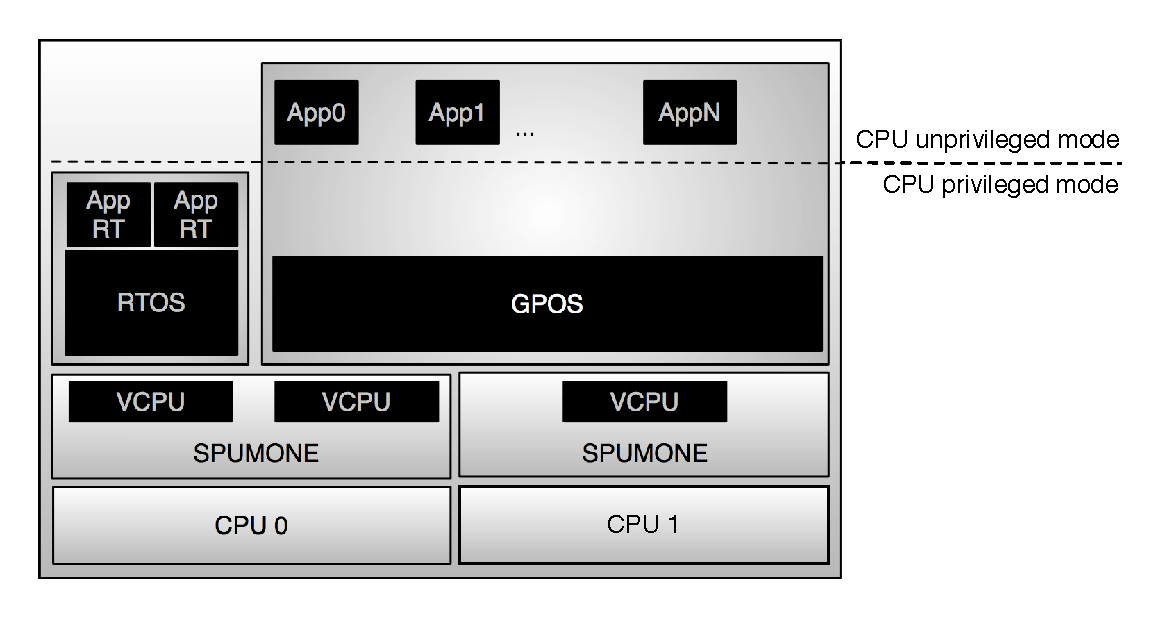
\includegraphics[width=.55\textwidth]{./chapter3/figures/spumone_multi}
\caption{SPUMONE's multicore Architecture. Adapted from \cite{hitoshi2011}.}
\label{fig:espumone_multi}
\end{figure}

In both SPUMONE versions (single and multicore), the authors chose better performance over reliability. Both RTOS and GPOS are complex software and can fail. For example, a faulty AppRT on the RTOS may compromise the whole system, because the hypervisor is at the same privilege level as the guest OS kernels. On the other hand, this approach decreases the number of hypercalls implemented in the guest OS, improving performance and maintainability.

In addition to the previously mentioned works, Mitake et al. \cite{mitake2012} proposed two new techniques to avoid the LHP problem (see Subsection \ref{subsection:holder}) in real-time virtualized systems using SPUMONE. These techniques rely on the VCPU migration among physical cores. The first technique called trap based migration consists in does not allow Linux to execute the kernel code on core 0 (see Figure \ref{fig:espumone_multi}). As the LHP is caused by the kernel's spinlocks, performing Linux kernel only on core 1 guarantee that the RTOS is performing concurrently with the Linux (see Figure \ref{fig:espumone_multi}). The second technique called on-demand migration consists in to migrate Linux from core 0 to core 1 when the RTOS executes on core 0 avoiding to execute the Linux and the RTOS on the same physical core. If the RTOS is addle, the Linux can perform on both cores. 


\section{XtratuM}
\label{section:XtratuM}

Crespo et al. \cite {xtratum2010} presented the XtratuM, a type 1 hypervisor specially designed for real-time embedded systems to meet temporal and spatial requirements of safety critical systems. In order to better fit real-time constraints, XtratuM was developed with the following a set of requisites: 

\begin{itemize}
\item data structures are static to allow for better control over the resources being used; 
\item XtratuM’s code is non-preemptive to make the code simpler and faster; 
\item all hypercalls are deterministic;
\item peripherals are managed by the VMs (directly mapped devices);  
\item interrupt occurrence isolation (when a VM is in execution only the interrupts related to it are enabled). 
\end{itemize}

\begin{figure}[!hbtp]
\centering
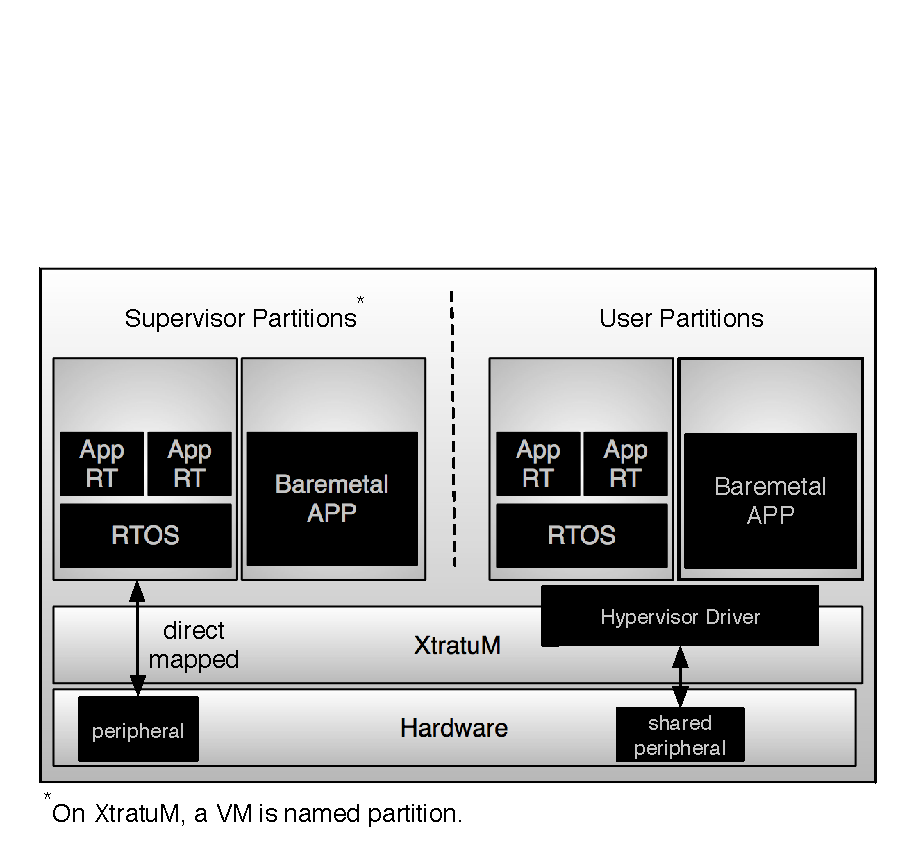
\includegraphics[width=.5\textwidth]{./chapter3/figures/XtratuM}
\caption{XtratuM's architecture. It is a type 1 hypervisor designed for safety critical systems. Adapted from \cite {xtratum2010}.}
\label{fig:XtratuM}
\end{figure}

Initially developed over x86, XtratuM now supports LEON2, LEON3, LEON4 (SPARC-V8 RISC \cite{sparkv8}) and ARM processor architectures. The hypervisor's overall architecture is shown in Figure \ref{fig:XtratuM}. In XtratuM, each VM is called a partition and each partition can support a RTOS or a bare metal application (GPOSs are not supported). There are two types of partitions: normal and system. Normal partitions have restricted functionality while system partitions can manage and monitor the state of the system and other partitions. Unlike SPUMONE, XtratuM  virtualizes not just the CPU and interrupts, but also some specific peripherals using para-virtualization. If there is no need to share a peripheral between two or more partitions, it can be directly mapped to the specific partition. When a peripheral needs to be shared between partitions, XtratuM implements a device driver to serialize the access and the guest OS must be modified in order to implement hypercalls to this device driver. 

In addition to previous work, Trujillo et al. \cite{trujillo2013} proposed the MultiPARTES: a project to support mixed critically integration for embedded systems based on virtualization techniques. It uses the XtratuM for virtualization purposes. MultiPARTES project resulted in a tool that allows for the application description using UML and additional annotations, like CPU time, memory, or bandwidth. The tool uses these descriptions to define a system partitioning and generate three outcome: source code, XtratuM configuration files, and system generation files. The authors claim that their approach accelerates the certification process for mixed-critical systems.


\section{L4 Microkernel Family based hypervisors}
\label{section:l4}

The microkernel concept reduces the OS kernel code to fundamental mechanisms and implements the remainder of the system services at the user level \cite{Liedtke1995}. The L4 microkernel was based on the L3 OS \cite{liedtke1993} developed by Liedtke to the x86 processor architecture. During his work at GDM and IBM, Liedtke modified the L3 to implement and test new ideas resulting in the L4. This initial development triggered an entire family of L4 based microkernels. Figure \ref{fig:timeline} summarizes the L4 microkernels family tree that resulted in embedded hypervisors. 

 

\begin{figure}[!hbtp]
\centering
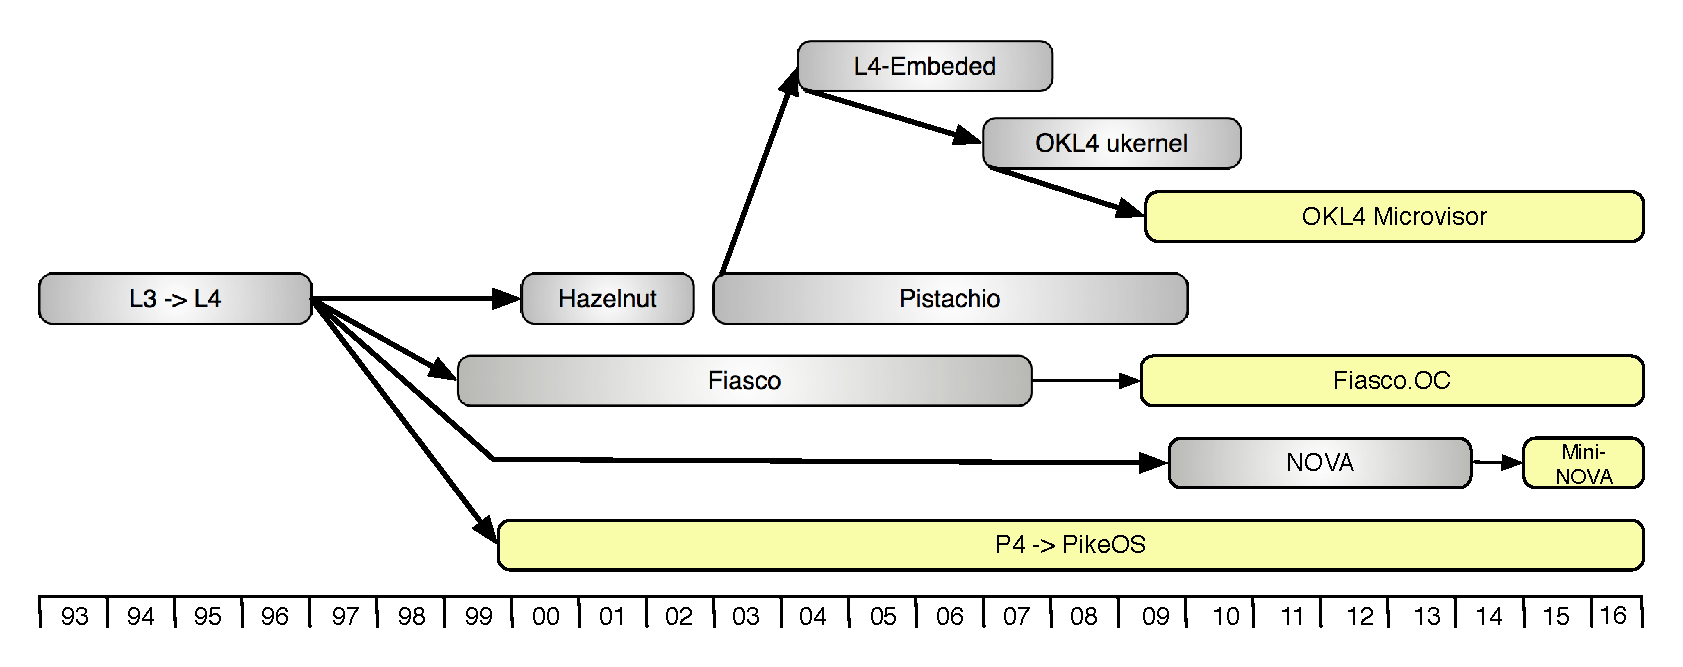
\includegraphics[width=.8\textwidth]{./chapter3/figures/l4-timeline}
\caption{Summarized L4 microkernel family tree that resulted in embedded hypervisors. Adapted from \cite{elphinstone2013}.}
\label{fig:timeline}
\end{figure}

GDM and IBM imposed a restrictive intellectual propriety for other researchers, forcing the University of Dresden to implement an x86 version of the L4 from scratch, called Fiasco. It was later renamed to Fiasco.OC. Liedtke moved to the University of Karlsruhe where he developed a version of the L4 supporting Pentium and ARM architectures, called Hazelnut. In 2001, it was implemented a new open-source kernel, called Pistachio, based on the previous version of L4. This kernel was written to x86 and PowerPC.  The NICTA Laboratory and the University of South Wales ported it to MIPS, Alpha, 64-bit PowerPC and ARM. NICTA created a fork of Pistachio, called L4-embedded, that was adopted by Qualcomm as an RTOS on wireless modems. The NICTA work resulted in a spin-off company called Open Kernel Labs for further support and development of the kernel. This company renamed L4-embedded OKL4 and developed the OKL4 Microvisor for virtualization purposes. PikeOS is another commercial clone of the original L4 that is certified for use in safety-critical avionics. NOVA is a open-source hypervisor based on L4 principles and designed for hardware-assisted virtualization on x86 platforms. Mini-NOVA is a port of the NOVA to the ARM Cortex-A9 using para-virtualization due to the absence of hardware support for virtualization on this processor. 


\subsection{OKL4 Microvisor}
\label{subsection:okl4}

The OKL4 Microvisor \cite{Heiser2010} was developed targeting mobile devices. Currently, it supports Linux, Android, Symbian and Windows Mobile OSs. The OKL4 powered the first commercial virtualized phone in 2009, named Motorola Evoke QA4. It executed two VMs on top of the OKL4 Microvisor: a Linux guest to handle the user interface and another guest for the BREW (Binary Runtime Environment for Wireless). 

Figure \ref{fig:okl4} shows OKL4's overall architecture. The microvisor is the only software layer that executes in the privileged mode while GPOSs, bare metal applications and even device drivers execute in the unprivileged mode. It has the ability to execute several GPOSs and bare metal applications concurrently. 

\begin{figure}[!hbtp]
\centering
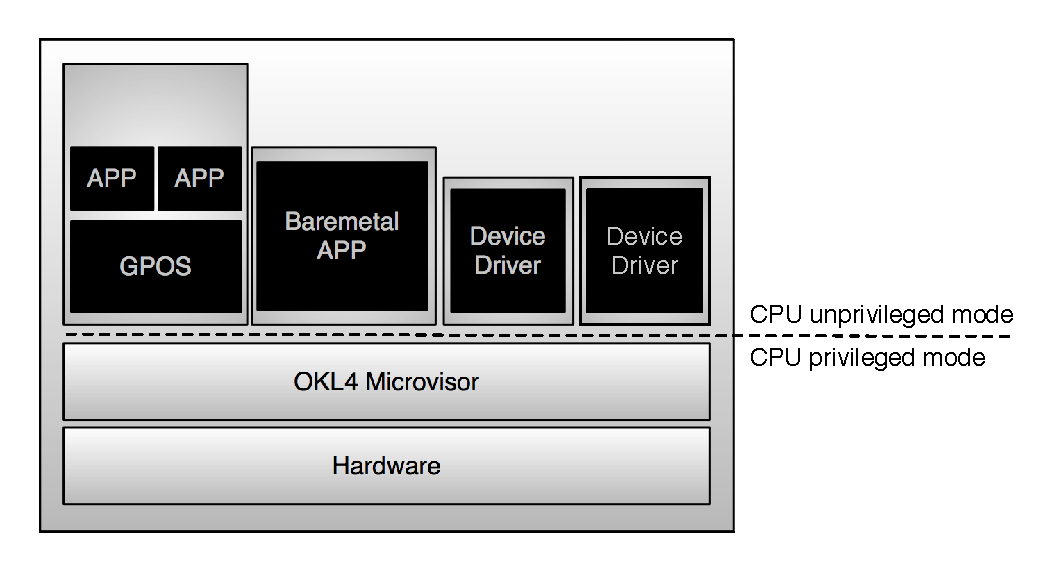
\includegraphics[width=.55\textwidth]{./chapter3/figures/okl4}
\caption{OKL4's architecture. It was developed targeting mobile devices supporting several mobile OSs, and it powered the first commercial virtualized phone in 2009.}
\label{fig:okl4}
\end{figure}

With OKL4 it is possible to execute both GPOS and a real-time environment on a single ARM processor, while providing high performance communication between them. This eliminates the need for a second ARM processor, which reduces the final cost and design complexity. 


\subsection{L4/Fiasco}
\label{subsection:fiasco}

The L4/Fiasco was developed as a clone of the original L4 kernel and adapted to provide virtualization on single-core x86 processors. Figure \ref{fig:fiasco} shows L4/Fiasco's architecture. L4Linux is a modified Linux kernel to support the L4/Fiasco's para-virtualization mechanism. It is mainly different from other hypervisors due to its  ability to map Linux kernel threads directly onto VCPUs. The L4Linux invokes hypercalls during kernel thread creation to allow to the L4/Fiasco to create VCPUs. However, this mechanism does not avoid the two-level scheduling problem because the Linux scheduler keeps mapping processes to Linux kernel threads. As is the case with other microkernels, device drivers are executed in user land. Additionally, L4/Fiasco supports RTOSs. 

%Confirmar se essa historia sobre o l4 Fiasco esta correta.

\begin{figure}[!hbtp]
\centering
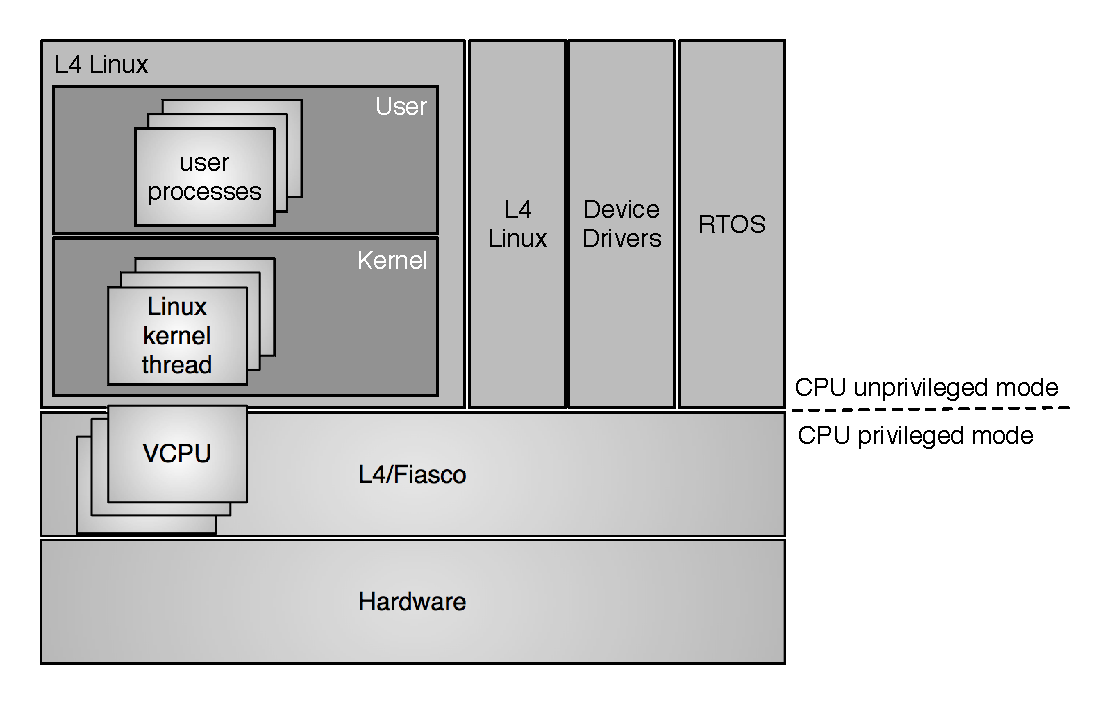
\includegraphics[width=.6\textwidth]{./chapter3/figures/fiasco}
\caption{Fiasco's architecture. The L4/Fiasco maps the L4Linux kernel threads directly to VCPUs.}
\label{fig:fiasco}
\end{figure}

Jungwoo et al. \cite{yang2011} proposed a compositional scheduling framework to deal with the two-level scheduling problem and extended  L4/Fiasco to support real-time constraints. L4Linux was modified to obtain the timing requirements from its internal processes and send them to the hypervisor through hypercalls. L4/Fiasco's scheduler implements a periodic task model and it uses the timing information from the guest OSs to meet the time constraints. This approach drastically reduces the number of deadline misses when compared to the original implementation. Additionally, it adds a small overhead that increases with the  number of threads. 


\subsection{PikeOS}
\label{subsection:pikeos}

PikeOS \cite{pikeos} is a proprietary microkernel developed by SYSGO AG\footnote{https://www.sysgo.com/} with support for virtualization. It was designed for safety-critical systems by implementing the concept of partitioning as defined by the ARINC 653 standard \cite{ARINC653}. Additionally, the standard determines the CPU time allocation across the partitions. The approach consists of a fixed cycle time in a specified order for a guaranteed duration. This allows for real-time guarantees, but it leads to a poor CPU utilization.  The microkernel has approximately 6,000 lines of code. It traps all interrupts and privileged instructions. Thus, it implements para-virtualization. Currently, it supports x86, PowerPCs and MIPS processors. 

\begin{figure}[!hbtp]
\centering
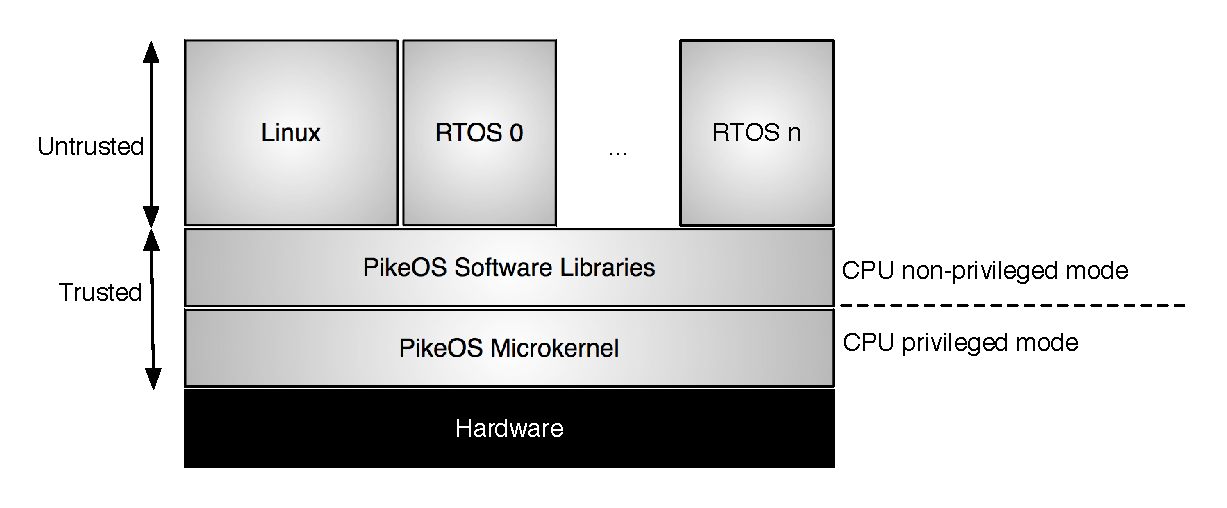
\includegraphics[width=.8\textwidth]{./chapter3/figures/pikeos}
\caption{PikeOS's architecture. It is a proprietary microkernel with support for virtualization designed to attend safety-critical systems.}
\label{fig:pikeos}
\end{figure}

Figure \ref{fig:pikeos} depicts the architecture of the PikeOS. The microkernel is the only software executed in CPU's kernel mode. The PikeOS software layers establish a set of partitions or VMs. Each partition can host a para-virtualized OS. The guest OSs are considered untrusted software and are kept isolated from each other. Finally, PikeOS supports inter-VM communication between guest OSs based on a mechanism defined by the ARINC standard. In this mechanism, the microkernel acts as a communication arbiter to manage message exchanges. 

\subsection{Mini-Nova}
\label{section:mini}

In 2010, Steinberg et al. \cite{Steinberg2010} proposed a hypervisor supporting the VT-x extensions on x86 architecture, called NOVA. Based on the NOVA hypervisor, Xia et al. \cite{Xia2015} suggested the use of the NOVA microkernel on an ARM-FPGA platform capable of managing reconfigurable hardware parts dynamically, but without support for virtualization. In the following work, Xia et al. \cite{tian2015} presented the Mini-NOVA, a type 1 embedded hypervisor for the ARM architecture using para-virtualization due to the absence of hardware support. 

The main difference in their approach is to  manage the coexistence of software and hardware computing resources. Thus, Mini-NOVA provides support for dynamic partial reconfiguration (DPR) to hardware tasks. According to the authors, the major challenge of this approach is to coordinate the hardware resources efficiently among the separate VMs. Security is another major concern, because the hardware tasks are shared among the guests. The solution adopts a centralized technique where a hardware task manager performs as a hypervisor service that manages the hardware. If a guest needs to execute a hardware task, it must require it using hypercalls. The evaluation demonstrated that the hardware can be efficiently managed with a short response latency and with a small overall latency. 


\section{M-Hypervisor}
\label{section:mhyper}

The M-Hypervisor \cite{rui2013} is a type 1 hypervisor supporting the Loongson 2f \cite{loogson2f} MIPS based processor. It is implemented by referencing the XtratuM's principles (see Section \ref{section:XtratuM}). Para-virtualization is adopted because Loongson 2f does not support the newer MIPS-VZ module. Hardware virtualization support is expected to be seen in the next generation of Loongson. Similar to XtratuM, the VMs are called partitions and support different OSs, like Linux and RTOSs. Real-time is supported through bare metal applications. The M-Hypervisor provides virtualization of the timer, interrupt, memory management, process switching and scheduling to ensure the real-time performance of high-level applications in the partitions and also temporal and spatial isolation. Based on the benchmarks, the authors claim that the M-Hypervisor can guarantee accurate real-time performance.


\section{Xvisor}
\label{section:xvisor}

Xvisor, shown in Figure \ref{fig:xvisor}, is an embedded hypervisor that supports both full-virtualization and para-virtualization\cite{patel2015}. It supports ARM virtualization extensions to provide full-virtualization and para-virtualization through optional VirtIO compatible device drivers. It can map interrupts directly to guests, allowing guest interrupts to be handled without the intervention of the hypervisor. Additionally, it provides memory isolation between hypervisor, guests and guest applications using the third privileged level from ARM's virtualization support. However, Xvisor has a poor support for MIPS processors since it only supports para-virtualization on the MIPS 24k processor model under the Qemu emulator.

\begin{figure}[!hbtp]
\centering
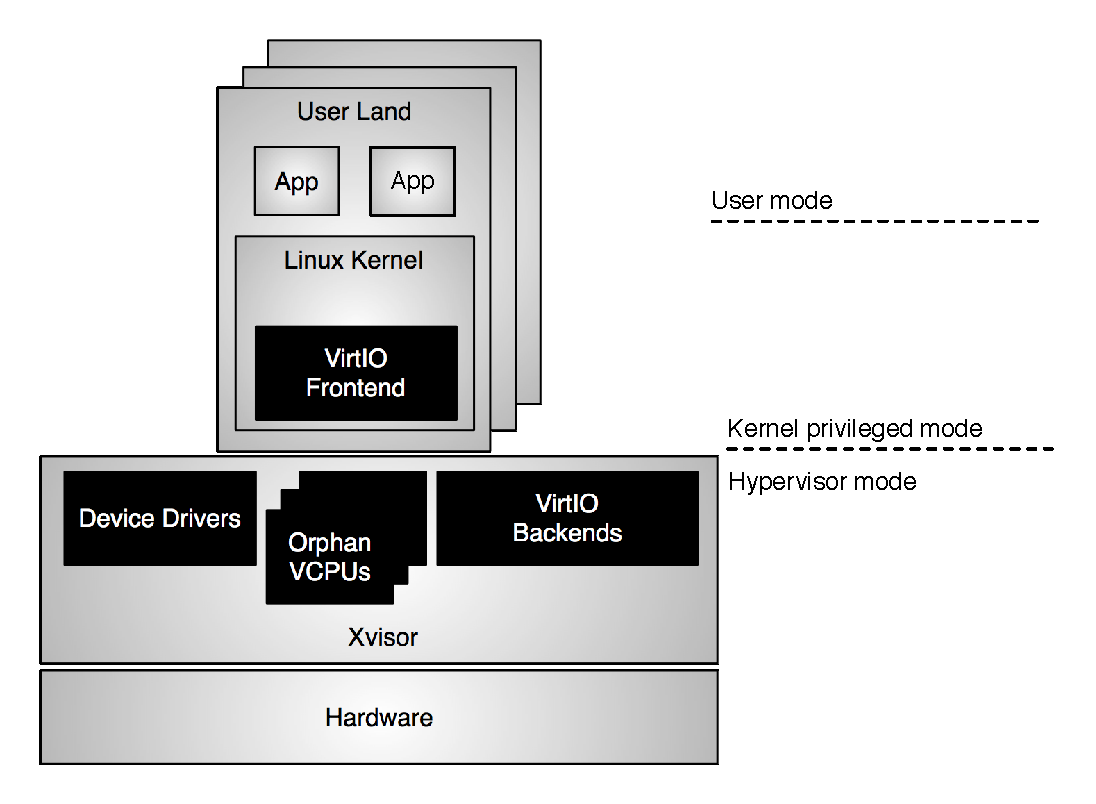
\includegraphics[width=.5\textwidth]{./chapter3/figures/xvisor}
\caption{Xvisor's architecture. The Xvisor hypervisor uses the third privileged level from ARM's architecture.}
\label{fig:xvisor}
\end{figure}

Xvisor implements the concept of Orphan VCPUs that executes background processing for device drivers and management purposes with the highest privilege. When compared to Xen or KVM, Xvisor has the advantage of having a single software layer where all virtualization related services are provided. For example, KVM depends on Qemu for device emulation and Xen depends on dom0 for I/O. Thus, the Xvisor's context switches are lightweight, resulting in instruction trap handling, host interrupts and guest I/O events. Also, the Xvisor's scheduler is per-CPU and does not do load balancing for multiprocessor systems. Instead, load balancing is performed by a distinct entity in Xvisor. 

\section{Embedded Hypervisors Comparison}
\label{section:comparative}

Table \ref{table:hypertable} is a comparison of the previously described embedded hypervisors and their key features. 

\begin{table}[!hbtp]
\caption{Embedded hypervisors' comparative table.}
\centering
\begin{tabular}{ p{2.5cm} p{3cm} p{3cm} p{3cm} p{3cm} l }
\hline\hline \\[-1.0ex]
\textbf{Hypervisor} & \textbf{Supported OSs} & \textbf{Architecture} & \textbf{Virtualization technique} & \textbf{Native Real-time support}\tablefootnote{Xen, KVM and L4/Fiasco can support real-time through modifications.} \\ [0.1ex]
\hline
Xen & Linux, Windows & ARM & PV, FV &  No \\ \hline
KVM & Linux, Windows & x86, ARM & PV, FV & No \\ \hline 
SPUMONE & Linux & SuperH-4A & PV & Yes \\ \hline
XtratuM & RTOSs & LEONx, ARM, & PV & Yes \\ \hline
OKL4 & RTOSs, Linux, Android & ARM, MIPS, x86 & PV & Yes\\ \hline
L4/Fiasco & Linux & x86(single-core) & PV & No\\ \hline
PikeOS & RTOSs & x86, PowerPC, MIPS & PV & Yes \\ \hline
Mini-NOVA & Linux, RTOSs & ARM & PV & Yes\\ \hline
M-Hypervisor & Linux, RTOSs & MIPS  & PV & Yes \\ \hline
Xvisor & Linux, RTOSs & ARM & PV/FV & Yes\\ \hline
\end{tabular}
\label{table:hypertable} 
\end{table}

The Xen hypervisor was developed for enterprise and desktop applications, as explained in Section \ref{section:xen}. However, recently it was ported to ARM processors. It does not support real-time natively. Instead, it requires modifications to improves the real-time responsiveness. Similar to Xen, KVM was recently ported to ARM processors and requires additional improvements in the Linux kernel to support real-time. All the other hypervisors presented were developed for embedded virtualization. However, with the exception of Xvisor, they were the first generation of embedded hypervisors. Thus, they share two important characteristics: lack of support for full-virtualization and lack of memory isolation between the guest's kernel and applications. Yet it is important to note that in SPUMONE the guest's kernel is executed in privileged mode along the hypervisor. Thus, it can keep the user applications isolated from each other, but the guest's kernel can access the hypervisor's memory space. Xvisor was designed to take advantage of the ARM virtualization support. Thus, it supports both full and para-virtualization and provides memory isolation between the hypervisor, guest kernel and guest applications. 

Tables \ref{table:footprintXenKvm} and \ref{table:footprintremain} compare the footprint of the hypervisors studied. Xen and KVM require the installation of additional elements to perform virtualization.  The installations column in Table \ref{table:footprintXenKvm} shows the different elements that must be installed with these hypervisors and their footprint. For example, Xen requires the Xen kernel, Dom0 and the Toolstack while KVM requires the Linux kernel and QEMU. Table \ref{table:footprintremain} compares the footprint of the remaining hypervisors.  
 
\begin{table}[!hbtp]
\centering
\caption{Footprint requirements for Xen and KVM.}
\label{table:footprintXenKvm}
\begin{tabular}{lccccc}
\hline \hline \\
                              & \multicolumn{3}{c}{\textbf{Installations}}                                    & \multicolumn{1}{l}{} \\ \\ \cline{2-4}
\multirow{2}{*}{\textbf{Xen}} & \textbf{Xen Kernel}        & \textbf{Dom0} & \textbf{Toolstack}   & \textbf{RAM}  & \textbf{footprint}\\
                              & 600KB \textgreater         & 3-4MB                    & 20MB \textless      & 180MB\textgreater   & 204MB\textless\\ \\\hline
\multirow{2}{*}{\textbf{KVM}} & \textbf{Host Linux zImage} & \textbf{QEMU}             & \multicolumn{1}{l}{} & \multicolumn{1}{l}{} & \textbf{footprint}\\
                              & 3-4MB                     & 20MB \textless           &                      & 20MB \textgreater & 44MB\textless   \\ \hline
\end{tabular}
\end{table}

Xen has a total footprint of roughly 204MB. KVM has a smaller footprint, but it requires a host Linux to execute. When compared to the configuration of modern computer servers, these requirements are modest. However, though they are used in embedded systems, their footprint may be unacceptable for many devices. 

\begin{table}[!hbtp]
\centering
\caption{Footprint requirements of the hypervisors when available.}
\label{table:footprintremain}
\begin{tabular}{llll}
\hline \hline \\
                     & \multicolumn{1}{c}{\textbf{kernel size}} & \multicolumn{1}{c}{\textbf{RAM Memory}} & \multicolumn{1}{c}{\textbf{footprint}}\\ \\ \hline
\textbf{SPUMONE}              & 30KB                                         &  - & >30KB\tablefootnote{The total memory needed by SPUMONE during its execution is unknown.}                                       \\
\textbf{Xtratum} & 8KB                                      & 16KB         & 24KB                            \\
\textbf{OKL4}                 & 48KB                                     & 78KB         & 126KB                           \\
%\textbf{L4/Fiasco}            &                                          &                                         \\
%\textbf{PikeOs}               &                                          &                                         \\
\textbf{Xvisor}               & 1-2MB                                    & 4-16MB       & 5-18MB                           \\
\textbf{Mini-NOVA}              & 40KB                                    & 20MB        & 20.04MB                         \\ \hline
\end{tabular}
\end{table}

Hypervisors developed for embedded systems typically present a smaller footprint than hypervisors for server virtualization. Unfortunately, some authors do not mention the memory requirement of their hypervisors. This is the case for L4/Fiasco, PikeOs and M-Hypervisor. The remaining of the hypervisors are shown in Table \ref{table:footprintremain}. Note that the footprint and RAM requirements can be quite different. For example, Xvisor has a footprint between 5 and 18MB. OKL4 has a footprint of only 126KB. SPUMONE's kernel requires 30KB each core in its multicore version. For example, in a dual-core processor SPUMONE will require 60KB. However, the amount of memory needed during its execution is unknown. Xtratum has the smallest footprint, requiring only 24KB during its execution.


\section{RT-Linux}
\label{section:rtlinux}

RT-Linux \cite{cottet2002} provides the capability of executing bare-metal tasks along a Linux OS. It is a kernel patch that adds a software layer with a real-time scheduler. From the point of view of the RT-Linux layer, the Linux kernel is a process that shares the processor with real-time tasks. Figure \ref{fig:rtlinux} shows RT-Linux's architecture. The I/O and interrupts subsystems of the Linux kernel are modified to communicate with the RT-Linux layer. This is similar to a para-virtualized hypervisor. The bare-metal tasks have priority over the Linux kernel and can access peripherals directly. Additionally, the Linux kernel will always be pre-empted to give priority to the real-time tasks. 

\begin{figure}[!hbtp]
\centering
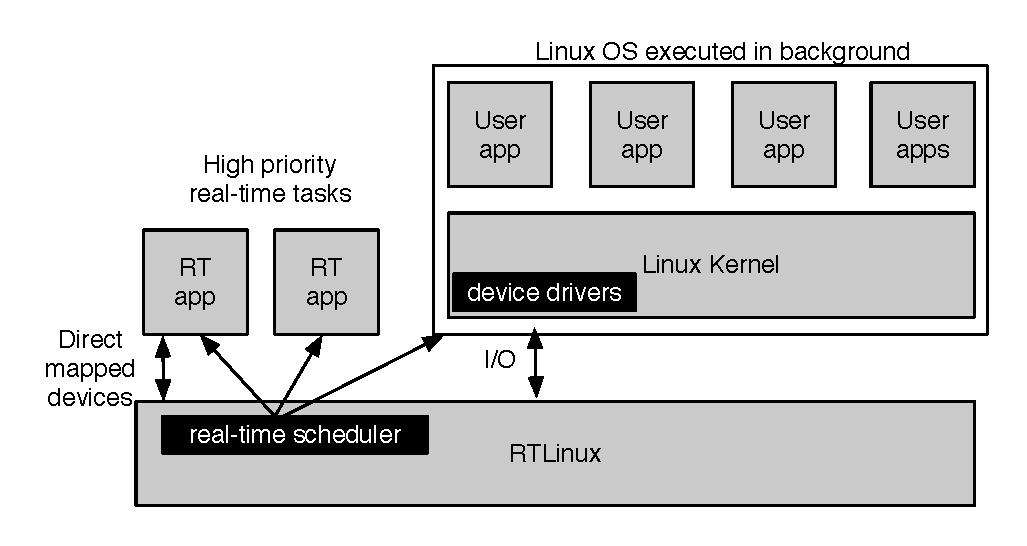
\includegraphics[width=.6\textwidth]{./chapter3/figures/rtlinux}
\caption{RT-Linux is a kernel patch that adds a software layer with a real-time scheduler and it makes the Linux kernel to share the processor with real-time tasks.}
\label{fig:rtlinux}
\end{figure}

RT-Linux's architecture is similar to a lightweight hypervisor, but without the capability of supporting multiple guest OSs. In fact, its objective is to improve the responsiveness of real-time tasks while maintaining the Linux software stack. The real-time tasks must be written using the RT-Linux API. Finally, shared memory can be used for communication between real-time tasks the Linux threads. 

\section{Final Considerations}
\label{section3:considerations}

This chapter presented the main hypervisors available for embedded virtualization. This study exposed the complexity of  embedded virtualization and the wide range of possible solutions. It was identified that real-time is an issue addressed frequently, since all mentioned hypervisors have some real-time support. In respect to Xen and KVM, the primary focus of the studied works is the issue of real-time improvements. These hypervisors have a deep dependency on the Linux OS, which makes it difficult to reduce their memory requirements. Thus, a recurrent challenge for hypervisors specially designed for embedded systems is to achieve a small footprint. To accomplish this goal, they avoid dedicating domains for I/O (in contrast  to Xen) and they implement the type 1 hypervisor model (unlike KVM).  Also, the presented hypervisors regularly do not meet common embedded system requirements. For example, XtratuM does not support GPOSs while SPUMONE cannot provide spatial isolation between guests. L4 based hypervisors support GPOSs and provide spatial separation but do not support full-virtualization. Para-virtualization is extensively adopted on embedded hypervisors. As seen in Table \ref{table:hypertable}, KVM and Xvisor are the only embedded hypervisors that support full-virtualization, but their support is limited to the ARM virtualization extensions. Chapter \ref{chapter:background} showed that hardware-assisted virtualization is a trend in embedded processors. Thus, it is inevitable for the further development on hypervisors to adopt full-virtualization even when combined with para-virtualization. This study makes it clear that an novel embedded virtualization model is required to take advantage of newer processors and to better fit embedded system needs.


%trabalho que precisam ser analizados

%XEN

%2012 - Credit-based Low Latency Packet Scheduling Algorithm for Real-time Applications 



%KVM/ARM: The Design and Implementation of the Linux ARM Hypervisor

%KVM

%NV-CFS: NVRAM-Assisted Scheduling Optimization for Virtualized Mobile Systems - http://ieeexplore.ieee.org/xpl/articleDetails.jsp?arnumber=7336257&queryText=KVM%20EMBEDDED&sortType=desc_p_Publication_Year&searchField=Search_All

%Responsive and Enforced Interrupt Handling for Real-Time System Virtualization - http://ieeexplore.ieee.org/xpl/articleDetails.jsp?arnumber=7299849&queryText=KVM%20EMBEDDED&sortType=desc_p_Publication_Year&searchField=Search_All

%Platform Device Assignment to KVM-on-ARM Virtual Machines via VFIO - http://ieeexplore.ieee.org/xpl/articleDetails.jsp?arnumber=6962282&queryText=KVM%20EMBEDDED&sortType=desc_p_Publication_Year&searchField=Search_All

%Processor virtualization on embedded linux systems - http://ieeexplore.ieee.org/xpl/articleDetails.jsp?arnumber=6924360&queryText=KVM%20EMBEDDED&sortType=desc_p_Publication_Year&searchField=Search_All

%SPUMONE

%A Light-Weighted Virtualization Layer for Multicore Processor-Based Rich Functional Embedded Systems - http://ieeexplore.ieee.org/xpl/articleDetails.jsp?arnumber=6195872&queryText=SPUMONE&sortType=desc_p_Publication_Year&searchField=Search_All

%Using Virtual CPU Migration to Solve the Lock Holder Preemption Problem in a Multicore Processor-Based Virtualization Layer for Embedded Systems - http://ieeexplore.ieee.org/xpl/articleDetails.jsp?arnumber=6300159&queryText=SPUMONE&sortType=desc_p_Publication_Year&searchField=Search_All


% l4 family three - http://www.disy.cse.unsw.edu.au/projects/kernel/

%l4 fiasco - http://moss.csc.ncsu.edu/~mueller/rt/rt11/readings/projects/g3/report3.pdf

% Implementation of Compositional Scheduling Framework on Virtualization 


%AUTOSTAR

%http://ieeexplore.ieee.org/xpl/login.jsp?tp=&arnumber=6871203&url=http%3A%2F%2Fieeexplore.ieee.org%2Fstamp%2Fstamp.jsp%3Ftp%3D%26arnumber%3D6871203

%Takumi Shimada1
%http://ieeexplore.ieee.org/stamp/stamp.jsp?tp=&arnumber=7396874

